\documentclass[border=10pt]{standalone}
\usepackage[svgnames]{xcolor}
\usepackage{amsmath}
\usepackage{pgfplots}
\pgfplotsset{compat=newest}
\usepackage[sfdefault]{FiraSans}
\usepackage{FiraMono}
\renewcommand*\familydefault{\sfdefault}
\begin{document}
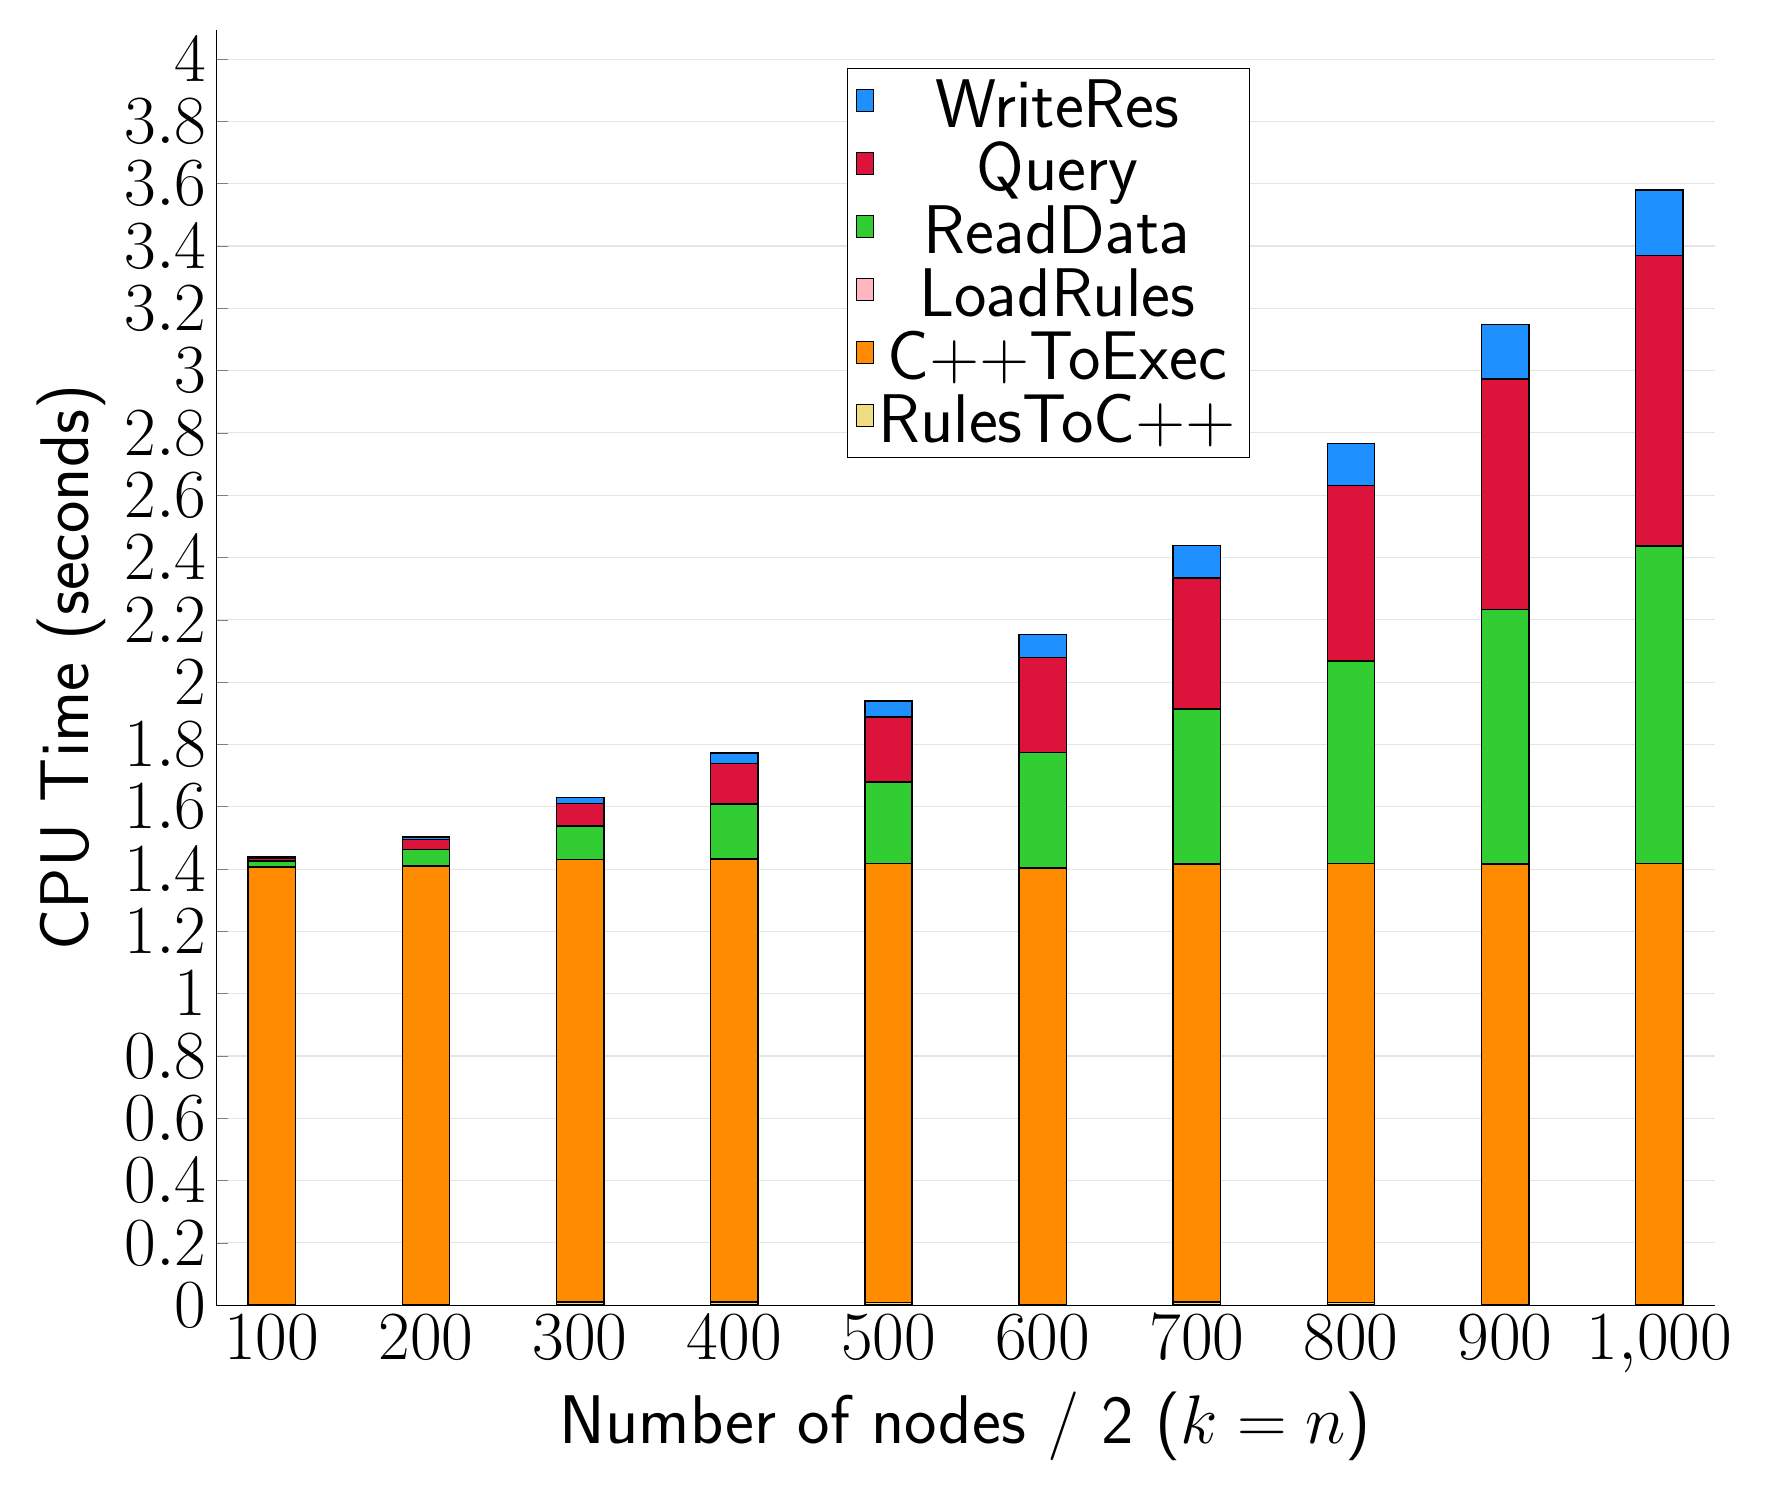
\begin{tikzpicture}
\begin{axis}[
   ybar stacked,
   width=1.7\textwidth,
   bar width=0.6cm,
   ymajorgrids, tick align=inside,
   major grid style={draw=gray!20},
   xtick=data,
   ymin=0, ymax=4.094,
   axis x line*=bottom,
   axis y line*=left,
   enlarge x limits=0.04,
   legend style={
       at={(0.69, 0.97)},
       anchor=north east,
       legend columns=1,
       font=\Huge,
   },
   ylabel={CPU Time (seconds)},
   xlabel={Number of nodes / 2 ($k=n$)},
   label style={font=\Huge},
   tick label style={font=\Huge},
]
\addlegendimage{fill=DodgerBlue, draw=black, line width=0.2pt}
\addlegendentry{WriteRes}
\addlegendimage{fill=Crimson, draw=black, line width=0.2pt}
\addlegendentry{Query}
\addlegendimage{fill=LimeGreen, draw=black, line width=0.2pt}
\addlegendentry{ReadData}
\addlegendimage{fill=LightPink, draw=black, line width=0.2pt}
\addlegendentry{LoadRules}
\addlegendimage{fill=DarkOrange, draw=black, line width=0.2pt}
\addlegendentry{C++ToExec}
\addlegendimage{fill=LightGoldenrod, draw=black, line width=0.2pt}
\addlegendentry{RulesToC++}
\addplot +[fill=LightGoldenrod, draw=black, line width=0.55pt] coordinates {
(100, 0.0020000000000000018)
(200, 0.0)
(300, 0.009999999999999995)
(400, 0.009999999999999995)
(500, 0.007999999999999997)
(600, 0.001999999999999999)
(700, 0.01)
(800, 0.007999999999999997)
(900, 0.001999999999999999)
(1000, 0.001999999999999999)
};
\addplot +[fill=DarkOrange, draw=black, line width=0.55pt] coordinates {
(100, 1.4040000000000004)
(200, 1.4100000000000001)
(300, 1.4200000000000004)
(400, 1.4220000000000002)
(500, 1.4100000000000001)
(600, 1.4020000000000004)
(700, 1.4060000000000001)
(800, 1.4100000000000004)
(900, 1.4140000000000001)
(1000, 1.416)
};
\addplot +[fill=LightPink, draw=black, line width=0.55pt] coordinates {
(100, 0.0001346)
(200, 0.00011800000000000001)
(300, 0.0001374)
(400, 0.00014399999999999998)
(500, 0.0001454)
(600, 0.0001418)
(700, 0.00011520000000000001)
(800, 0.0001534)
(900, 0.00010940000000000002)
(1000, 0.000145)
};
\addplot +[fill=LimeGreen, draw=black, line width=0.55pt] coordinates {
(100, 0.0198566)
(200, 0.05334680000000001)
(300, 0.10876440000000001)
(400, 0.17591659999999998)
(500, 0.2620292)
(600, 0.3693432)
(700, 0.49834759999999995)
(800, 0.6498196)
(900, 0.8174888000000001)
(1000, 1.0193820000000002)
};
\addplot +[fill=Crimson, draw=black, line width=0.55pt] coordinates {
(100, 0.0102198)
(200, 0.031269000000000005)
(300, 0.07122959999999999)
(400, 0.13089)
(500, 0.20729039999999999)
(600, 0.30528380000000005)
(700, 0.42031919999999995)
(800, 0.5629852)
(900, 0.7399180000000001)
(1000, 0.9317495999999998)
};
\addplot +[fill=DodgerBlue, draw=black, line width=0.55pt] coordinates {
(100, 0.0031572)
(200, 0.008686)
(300, 0.0191262)
(400, 0.033800399999999994)
(500, 0.0522382)
(600, 0.074781)
(700, 0.10376099999999999)
(800, 0.1349664)
(900, 0.1737374)
(1000, 0.2103446)
};
\end{axis}
\end{tikzpicture}

\end{document}
